% !TeX encoding=utf8
% !TeX spellcheck=de-DE
% !TeX root=../UID_Project_Documentation.tex

\section{Ideation}

Bei den Sketches haben wir uns grundlegend überlegt, wie die App die Anforderungen der potenziellen Nutzer, die durch unsere Personas repräsentiert werden, gelöst werden könnten. Ein wichtiger Punkt dabei ist es den Spagat zwischen der unterschiedlichen Technikaffinität der Personas zu bedienen. Beispielsweise sollen so wenig wie möglich Kognitionsfehler bei den Nutzern entstehen und auch bei erfahrenen Nutzern so wenig wie möglich Routinefehler. Die Sketches stellen Lösungen für die Probleme der Personas dar, die in die Prototyping Phase des UCD Prozess einfließen, um den Prototypen zu gestalten. Eine weitere Herausforderung einer News-App ist, dass sehr viel Inhalt auf übersichtliche Art und Weise auf sehr begrenztem Platz untergebracht werden muss.

\subsection{Sketch 1}

\begin{figure}[h]
  \centering
  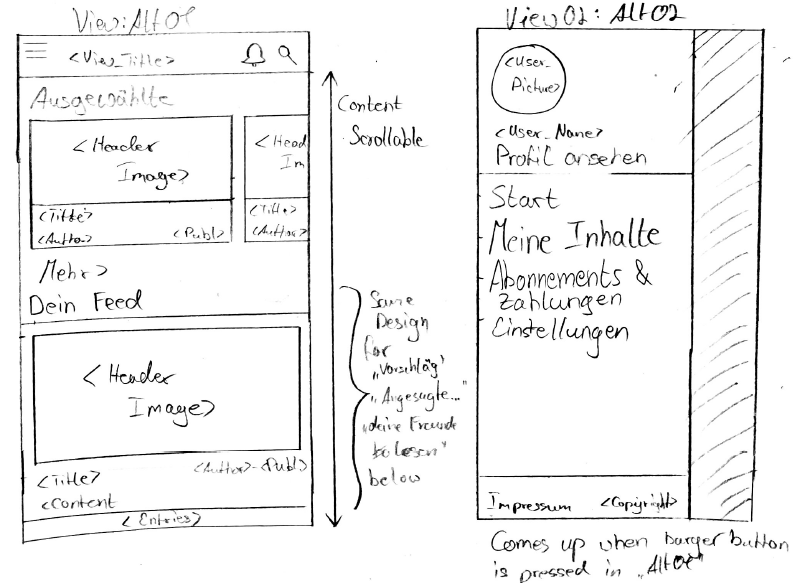
\includegraphics[width=\textwidth]{sketches 01}
  \caption{Sketch 1}
  \label{fig:sketch-01}
\end{figure}

Dieser Sketch verbindet Funktionsumfang und Übersichtlichkeit in hohem Maße, sodass daraus ein gesamtheitlich schlankes, aber intuitives Bedienkonzept resultiert. Besonders hervorzuheben ist aber der dargestellte Homescreen, sowie der Aufbau des Burgermenüs, an denen wir uns für den Prototypen orientieren möchten. Auf dem Homescreen befinden sich so verschiedene Gruppen von Artikeln, wie zum Beispiel \enquote{dein Feed} oder \enquote{Ausgewählte}, die es ermöglichen, eine Mehrzahl an Artikeln logisch strukturiert darzustellen.

\subsection{Sketch 2}

\begin{figure}[h]
  \centering
  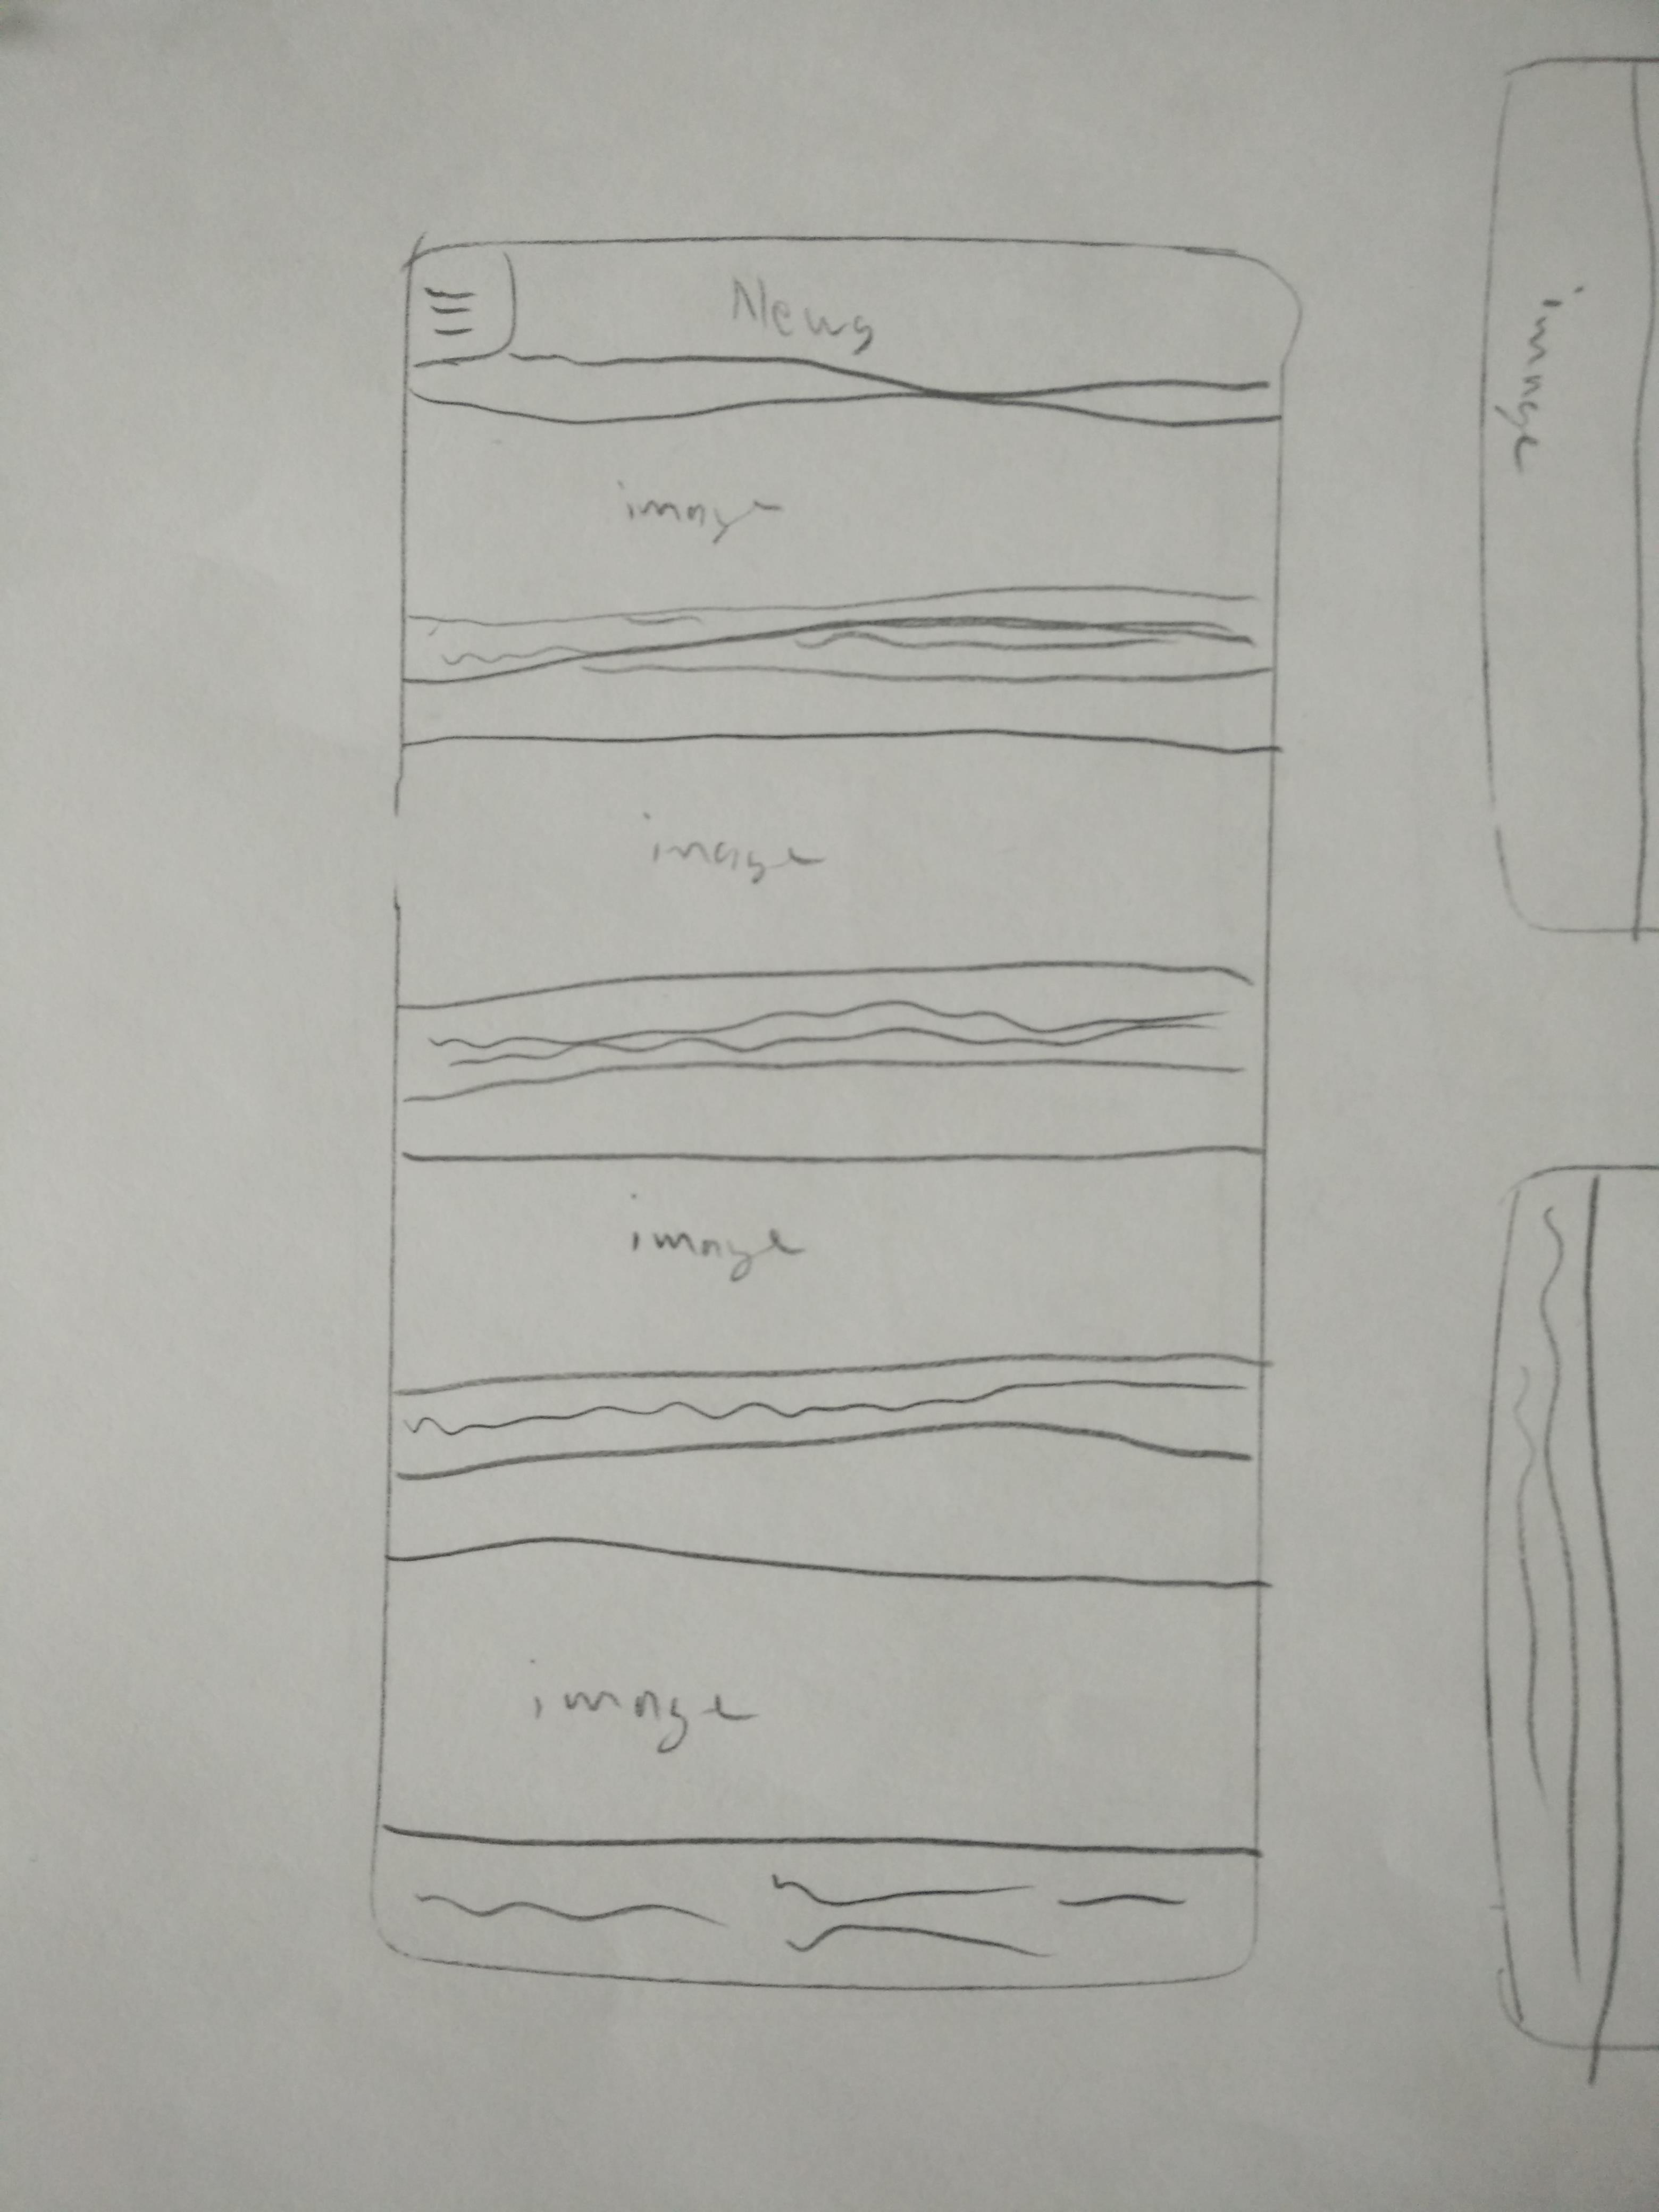
\includegraphics[height=\textheight/2]{sketches 02}
  \caption{Sketch 2}
  \label{fig:sketch-02}
\end{figure}

Dieser Sketch wurde ausgewählt, weil er enorm Sektminimalistisch ist, sodass der kleine Screen eines mobilen Gerätes maximal viel Inhalt bieten kann, da kein Platz für Navigationsleisten in Anspruch genommen wird. Damit einher geht auch ein hoher Grad an Übersichtlichkeit. Problematisch ist aber einerseits, dass trotz nicht vorhandener Menüleiste aufgrund der großen Bilder recht wenig Text untergebracht werden und andererseits, dass zu sämtlichen anderen Screens beziehungsweise Funktionalitäten nur umständlich über das \enquote{Burgermenü} navigiert werden kann. Dies ist wenig intuitiv und könnte den User sehr schnell von unserem Produkt abringen, da er nicht auf den ersten Blick findet, was er sucht und er den Funktionsumfang der App schwer einschätzen kann. Gerade beim erstmaligen öffnen der App würde dies möglicherweise viele Interessenten dazu bringen, die App sofort wieder zu deinstallieren, zumal der Sketch designmäßig recht pragmatisch und wenig ausgefeilt wirkt. Die Stärke dieses Sketches ist also gleichzeitig auch seine größte Schwäche. Er erinnert uns aber daran, platzsparend mit Navigationselementen umzugehen.

\subsection{Sketch 3}

\begin{figure}[h]
  \centering
  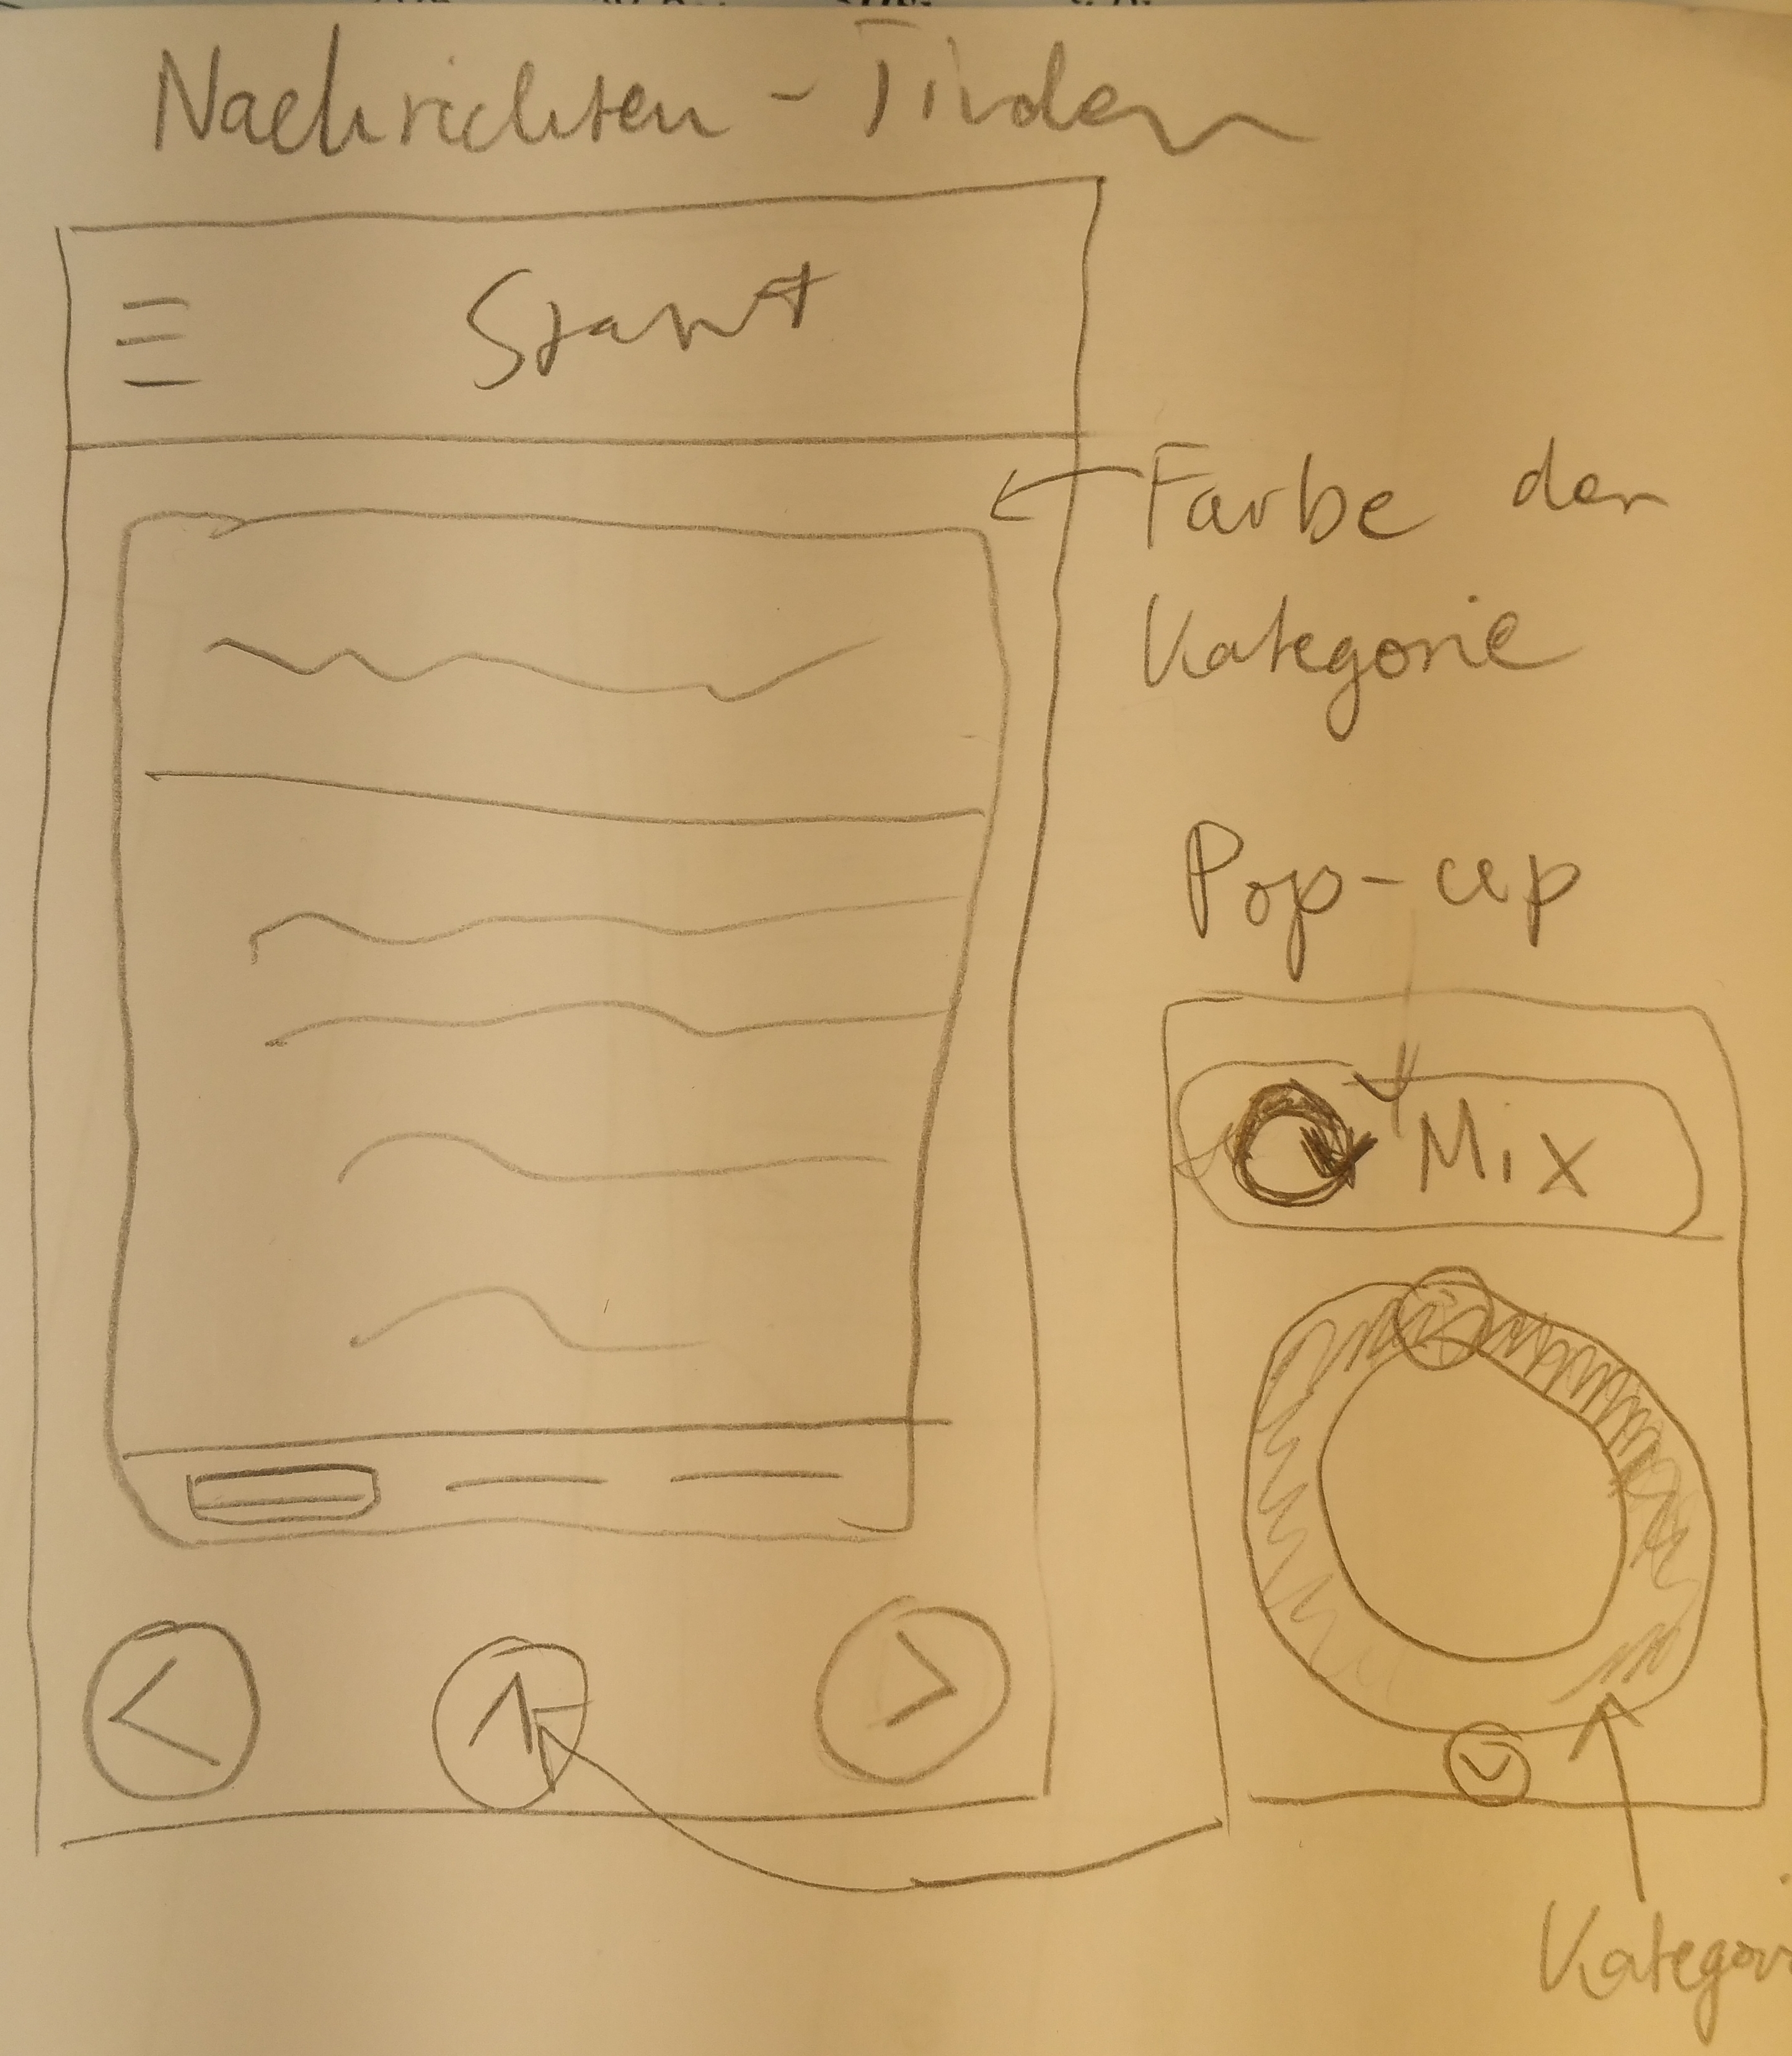
\includegraphics[height=\textheight/2]{sketches 03}
  \caption{Sketch 3}
  \label{fig:sketch-03}
\end{figure}

Dieser Sketch bringt ein abweichendes, aber sehr interessantes Bedienkonzept ein, nämlich eines, das sich stark an der berühmten \enquote{Tinder}-App orientiert. Dieses möchten wir auf jeden Fall in die Explore-Funktion unserer App integrieren, da dies ein Feature darstellt, welches bisher keine andere App dieses Genres bietet und vor allem das jüngere Publikum ansprechen dürfte. Aber auch für ältere Personen ist es ein leicht zu verstehendes, innovatives Konzept.

\subsection{Sketch 4}

\begin{figure}[H]
  \centering
  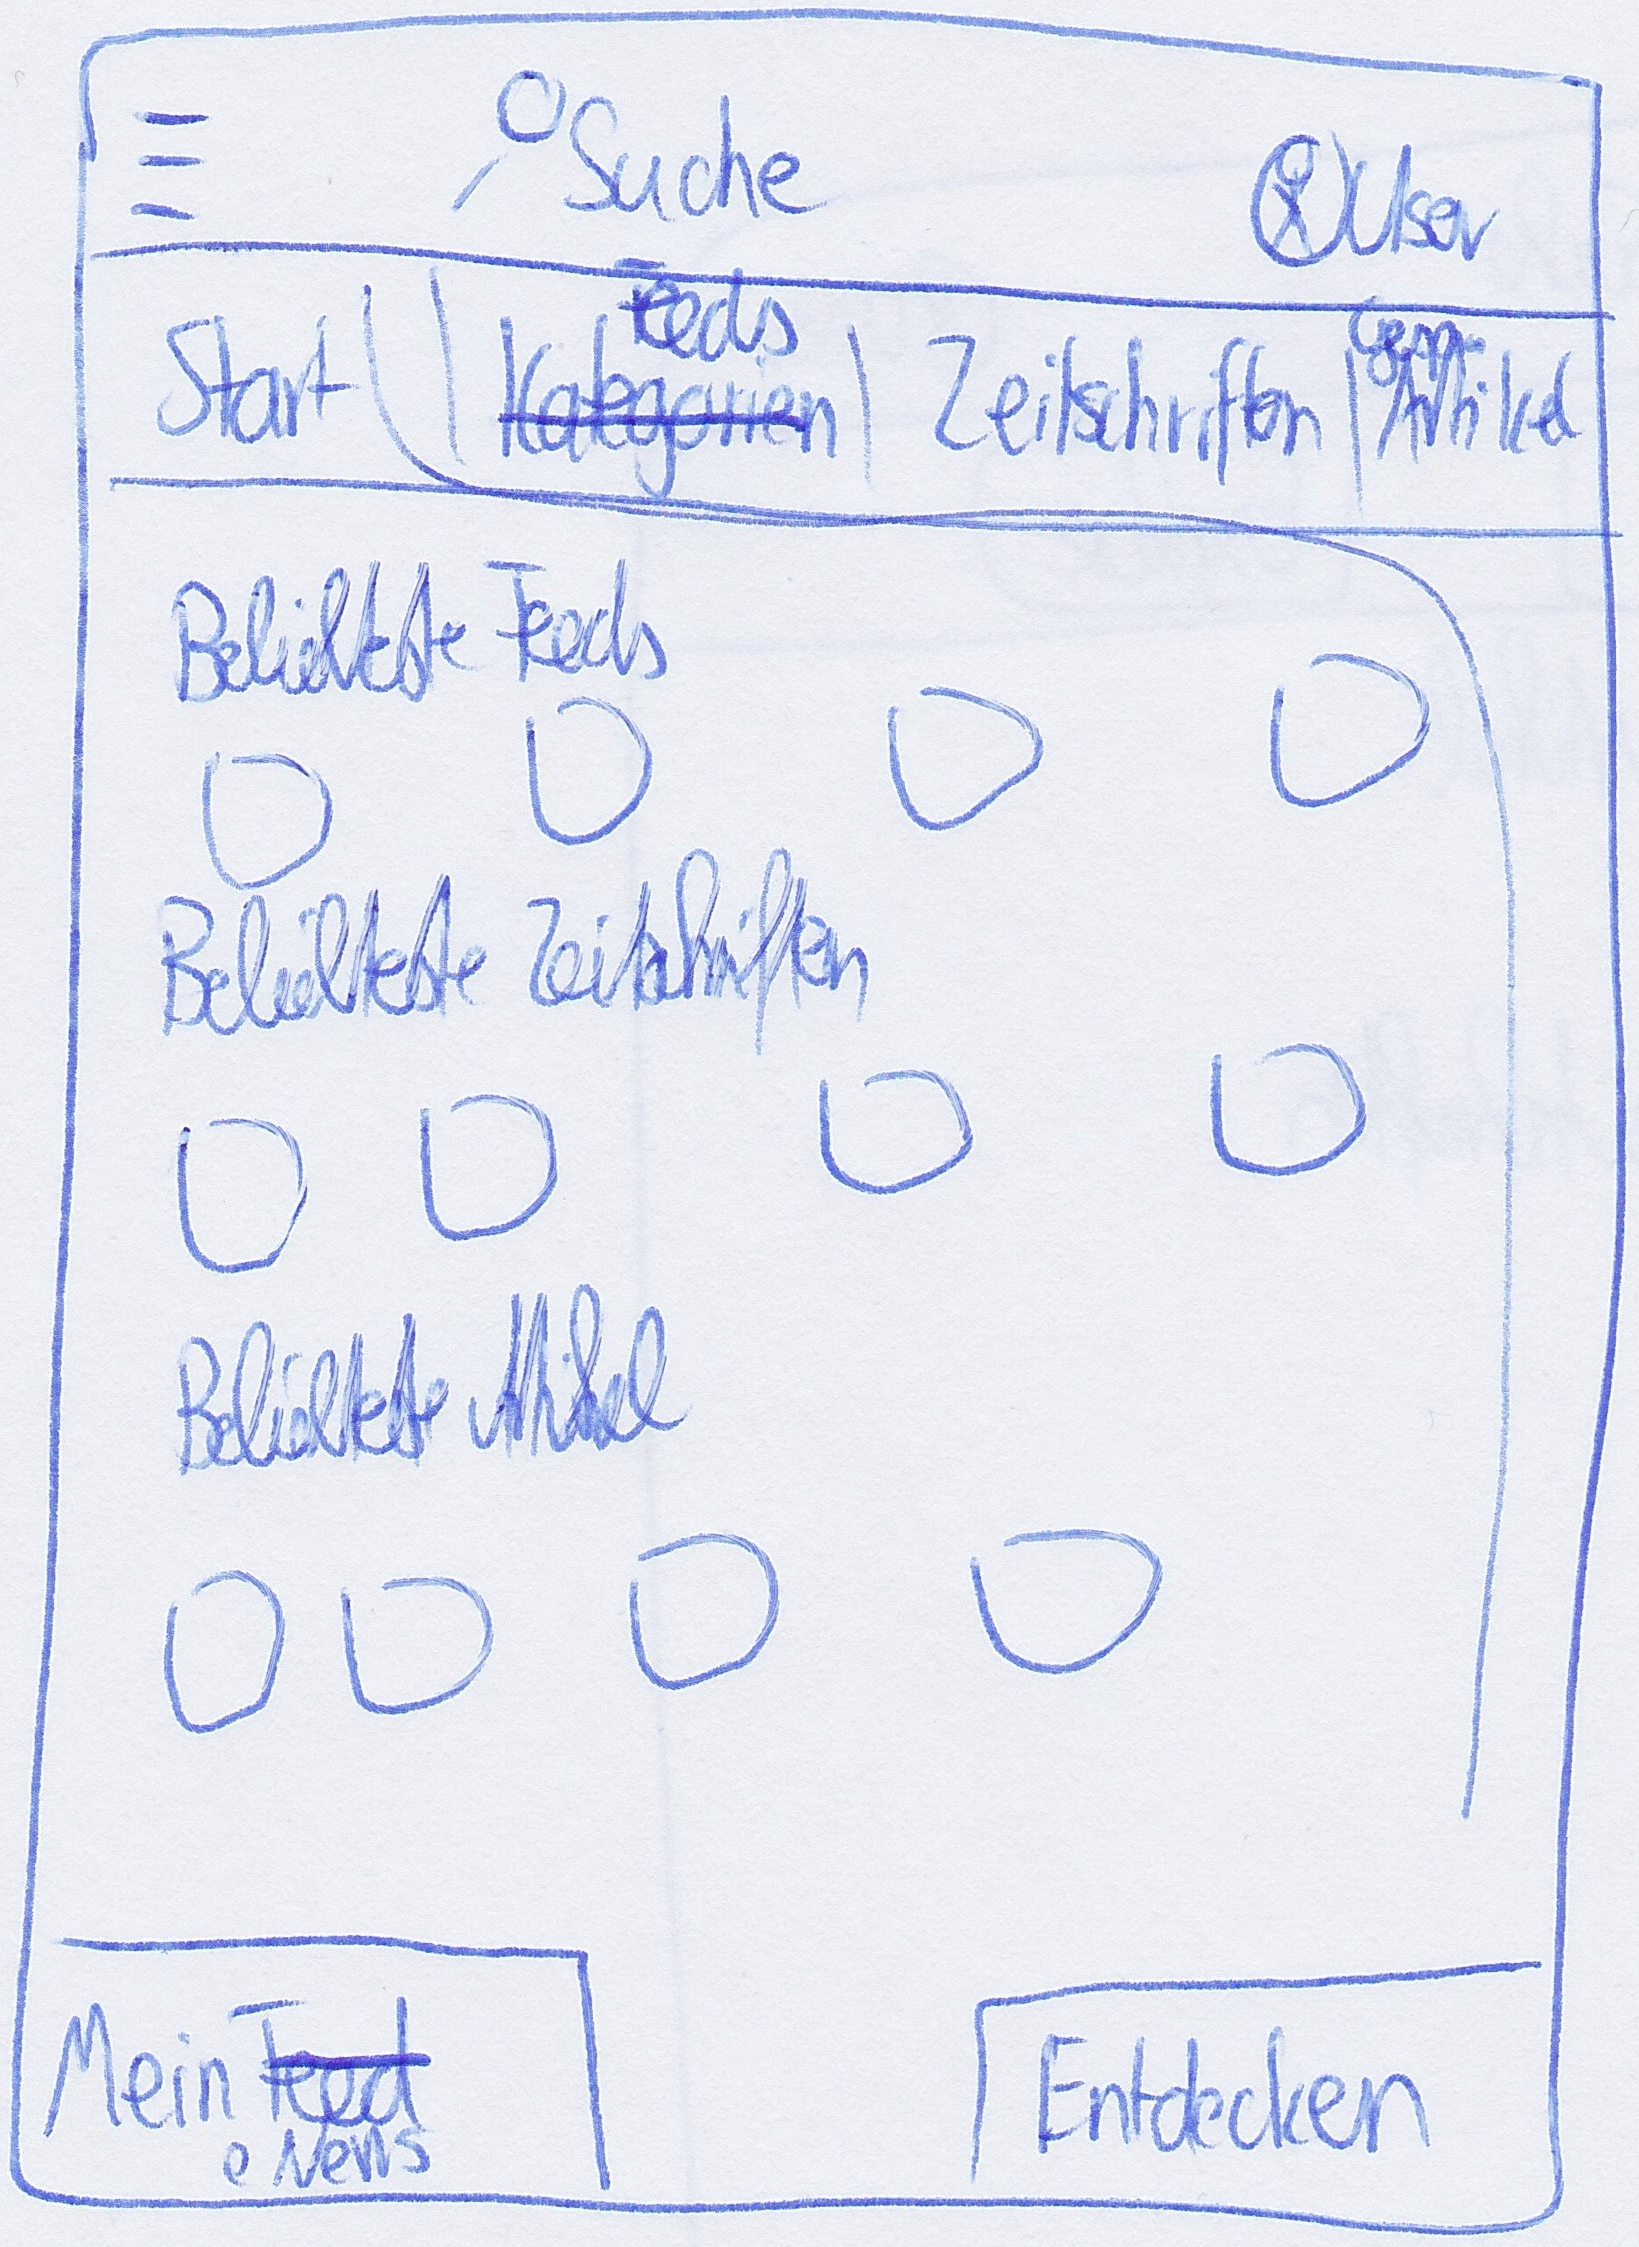
\includegraphics[height=\textheight/2]{sketches 04}
  \caption{Sketch 4}
  \label{fig:sketch-04}
\end{figure}

Dieser Sketch bringt einen hohen Grad an Funktionalität, sowie eine Navigationsmöglichkeit über Tabs ein. Problematisch an ihm sind die vielen Navigationselemente (Navigationsleiste unten, Tabs, Profil, Suche, Burgermenü), sodass möglicherweise die Übersichtlichkeit verloren geht und der User zunächst überfordert ist. Die Idee der einzelnen Tabs möchten wir aber auf jeden Fall in unseren Prototypen übernehmen, da sie mehrere Vorteile gegenüber anderen Navigationskonzepten besitzen. Unter anderem ist diese Form der Navigation schon aus vielen anderen Apps bekannt, sodass der User sich von Beginn an recht heimisch fühlen dürfte. Weiterhin suggerieren Tabs schon beim ersten Aufruf der App die Kernfunktionalitäten und geben ihr somit auf verständliche Weise Struktur. Zuletzt ist die Navigation mit ihnen auch sehr zügig möglich.
